\section{Einleitung}

''Ärzte und Zahnärzte haben den Anspruch in Ihren Praxen ein Rufsystem einzusetzen.
Dieses Rufsystem ermöglicht, dass der behandelnde Arzt über einen Knopfdruck Hilfe anfordern oder Behandlungsmaterial bestellen kann.''\cite{aufgabenstellung}
Mit diesem Projekt wurde ein cloudbasiertes Praxisrufsystem konzipiert und umgesetzt.
Dazu wurde das im Vorgängerprojekt ''IP5 Cloudbasiertes Praxisrufsystem'' umgesetzte Praxisrufsystem erweitert.
Das erweiterte System ermöglicht es Benachrichtigungen zu versenden und Sprachverbindungen zwischen Teilnehmern aufzubauen.
Als Benutzeroberfläche dient dabei eine native iOS Applikation.
Folgende Abbildungen zeigen die Startseite der iOS Applikation (Abbildung 1.1) sowie die Ansicht während eines aktiven Gruppenanrufs (Abbildung 1.2).

\begin{figure}[h]
    \centering
    \begin{minipage}[b]{0.4\textwidth}
        \fbox{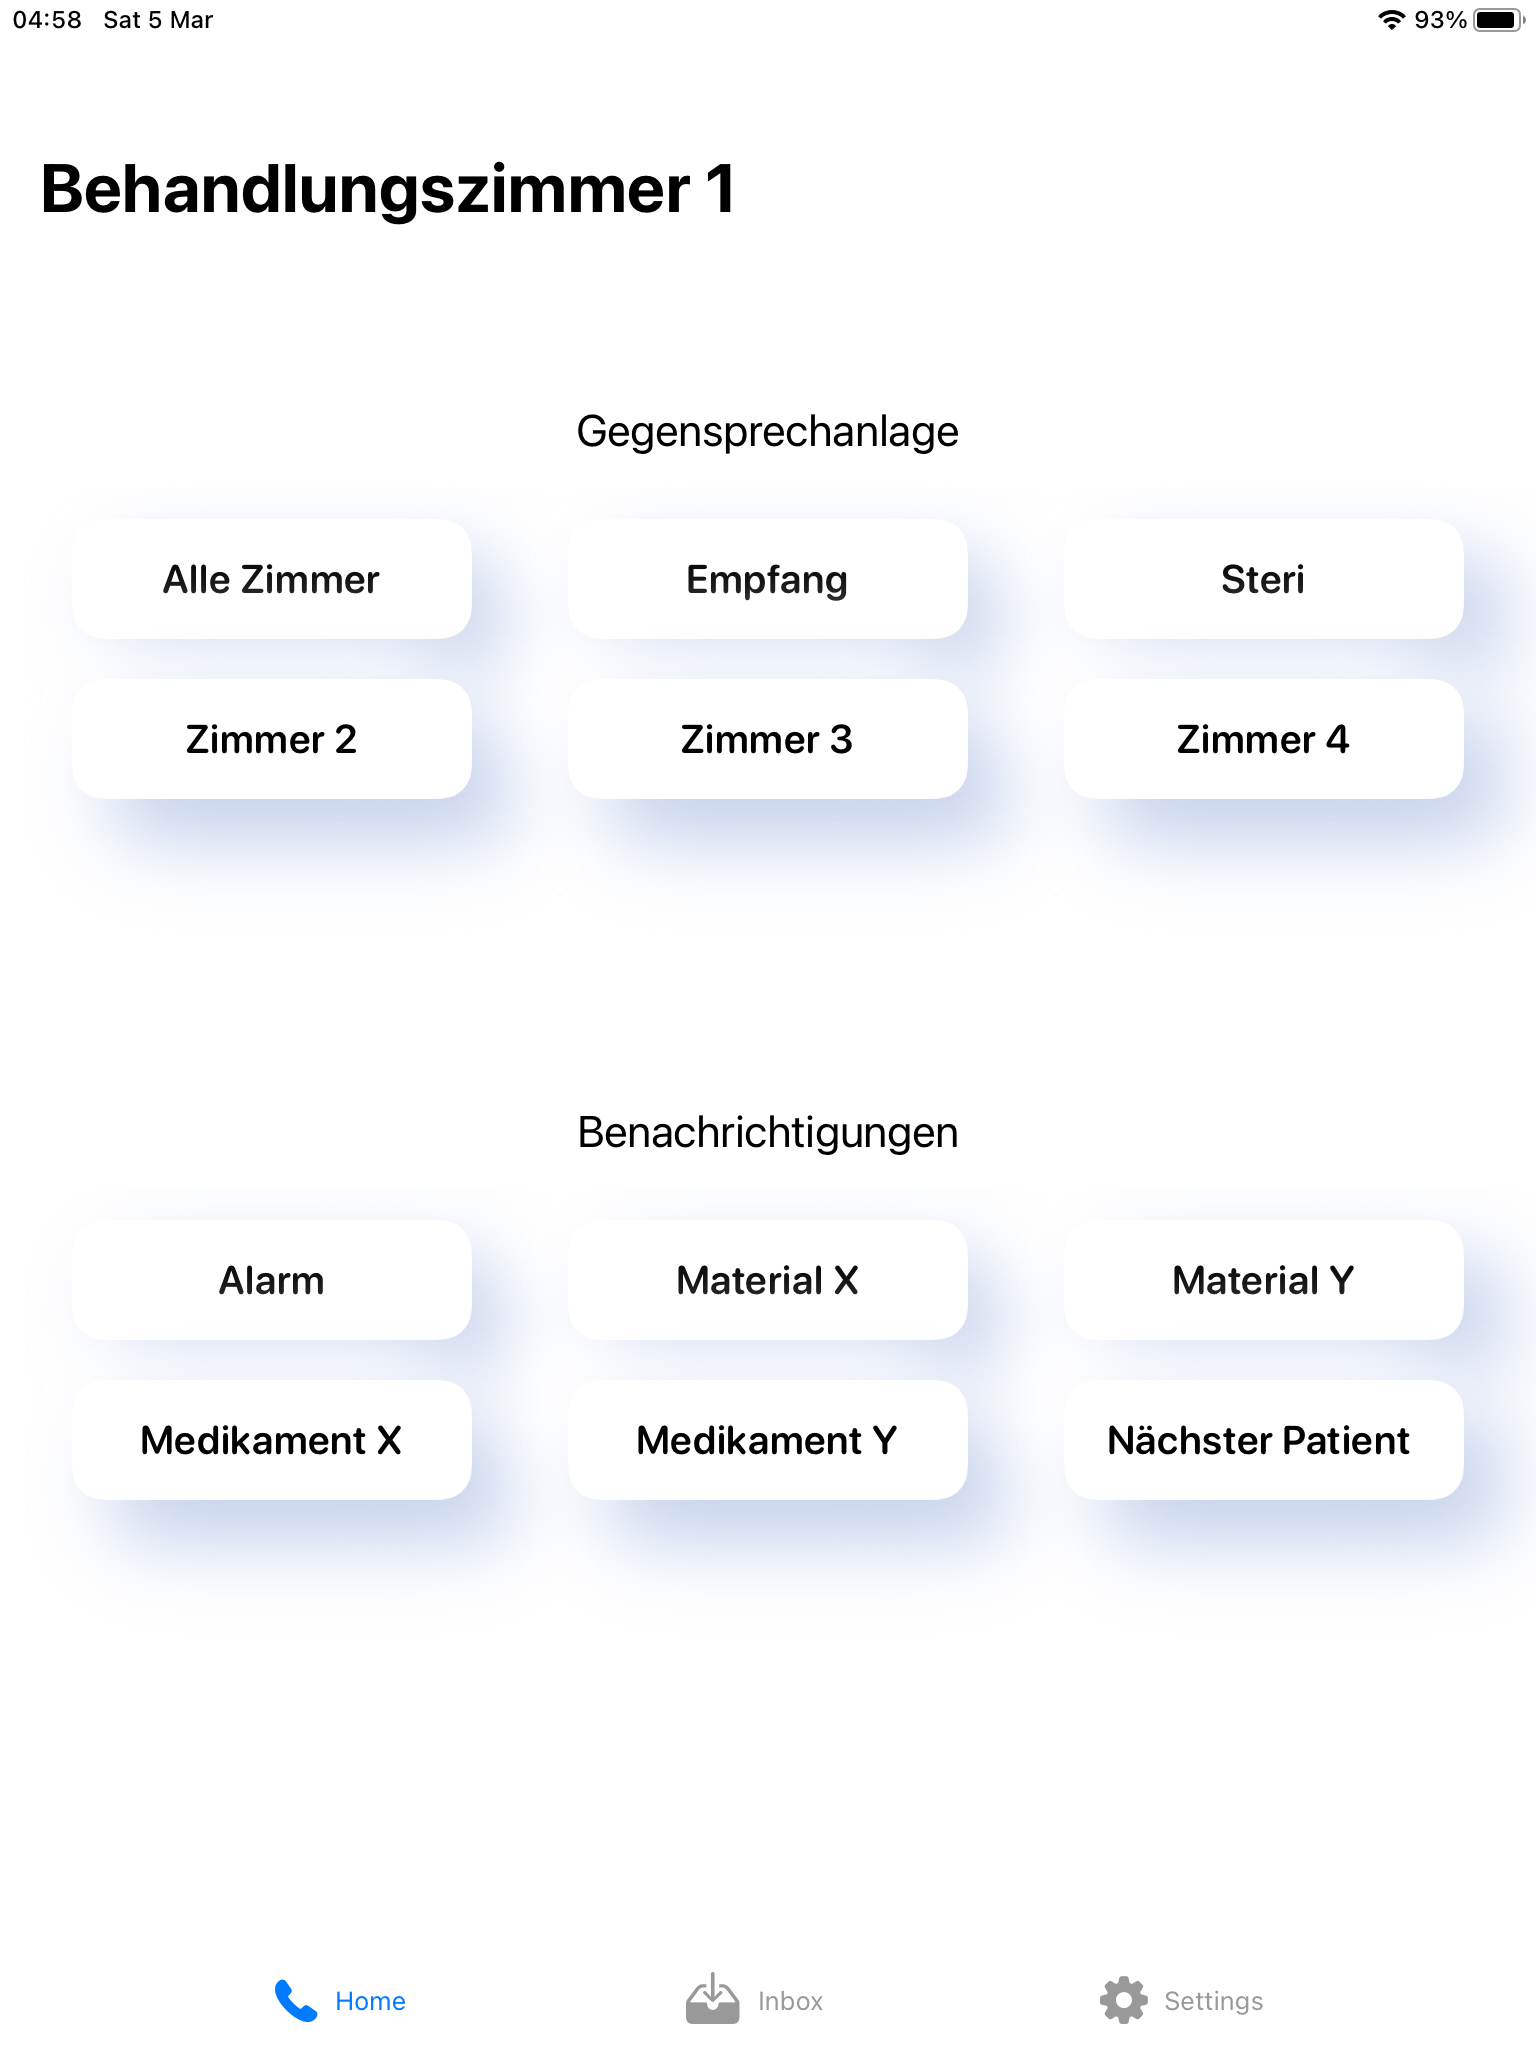
\includegraphics[width=\textwidth]{graphics/screenshots/app/home}}
        \caption{Praxisruf Startseite}
    \end{minipage}
    \hfill
    \begin{minipage}[b]{0.4\textwidth}
        \fbox{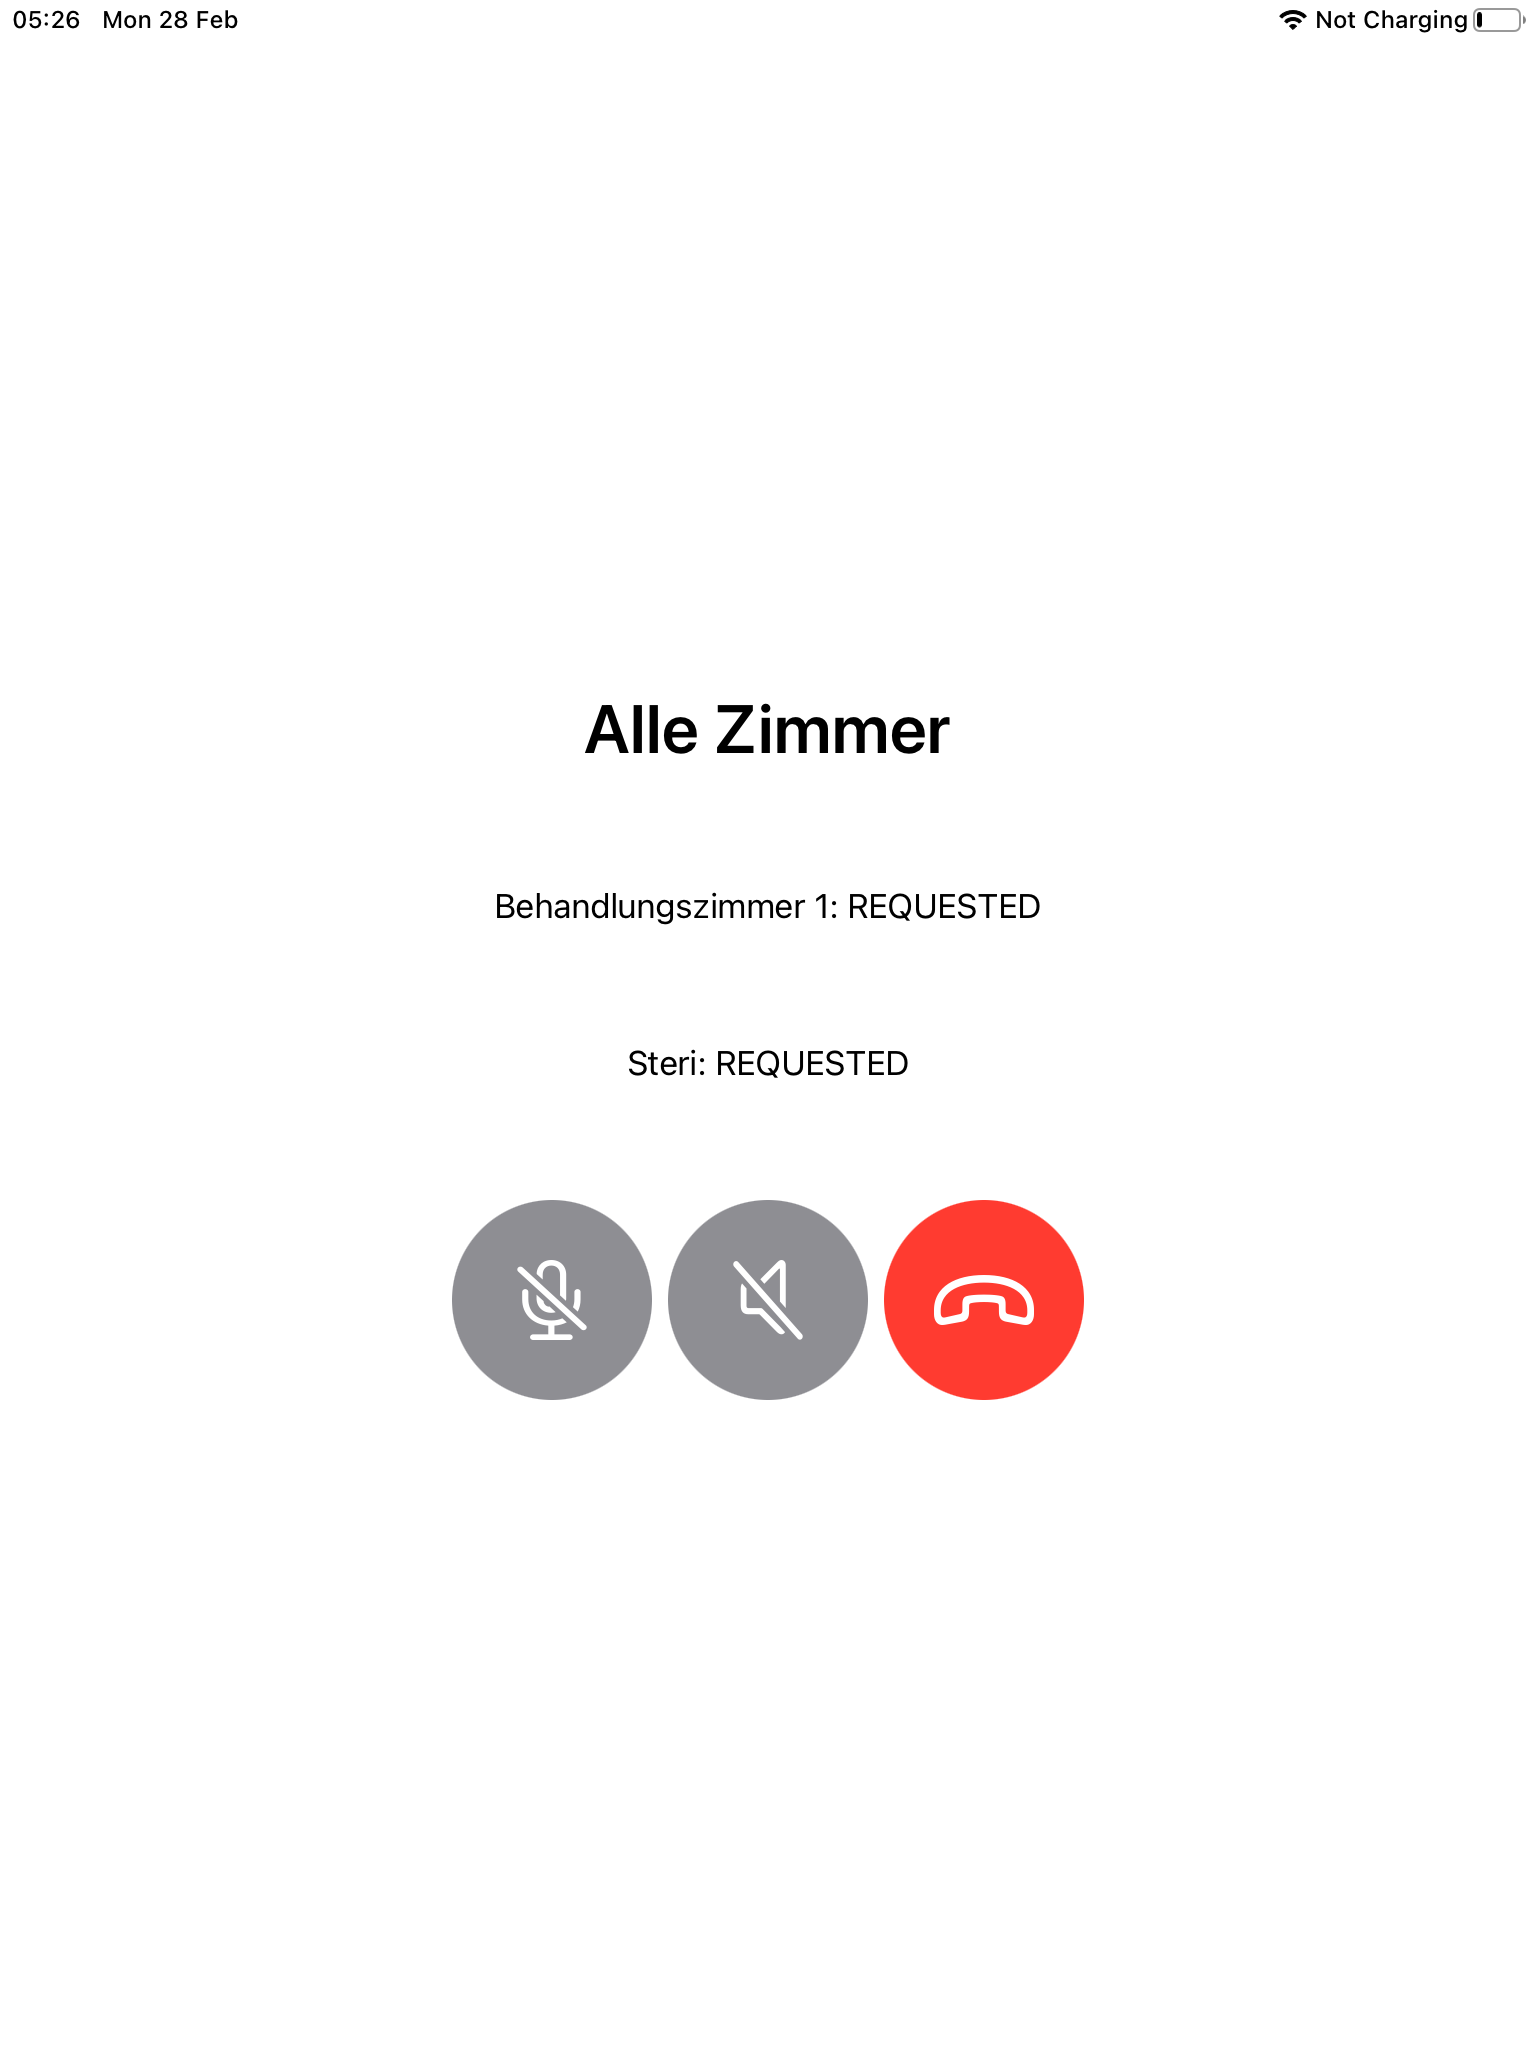
\includegraphics[width=\textwidth]{graphics/screenshots/app/call}}
        \caption{Aktiver Anruf}
    \end{minipage}
    \label{fig:MobileClient-ScreensIntroduction}
\end{figure}

Auf der Startseite der Applikation können per Knopfdruck Benachrichtigungen versendet und Sprachverbindungen gestartet werden.
Empfangene Benachrichtigungen werden als Push-Benachrichtigung angezeigt und in einer Inbox gesammelt.
Bei entsprechender Konfiguration wird zudem der Inhalt von empfangenen Benachrichtigungen automatisch vorgelesen.
Sprachverbindungen können zwischen zwei oder mehr Teilnehmern aufgebaut werden.
Das System unterstützt sowohl private Gespräche als 1:1 Verbindungen wie auch Gruppenunterhaltungen als 1:N Verbindungen.

Welche Buttons und damit welche Benachrichtigungen und Sprachverbindungen zur Verfügung stehen, wird durch Praxisadministratoren konfiguriert.
Die Konfiguration von Buttons für Sprachverbindungen beinhaltet, mit welchen Empfängern eine Verbindung aufgebaut wird.
Die Konfiguration von Buttons für Benachrichtigungen definiert den Inhalt der Benachrichtigung, welche Empfänger sie erhalten und ob die Benachrichtigung vorgelesen wird.
Für die Verwaltung dieser Konfiguration kann durch eine Weboberfläche vorgenommen werden.
Abbildung 1.3 zeigt die Übersicht verfügbarer Benachrichtigung in dieser Weboberfläche.

\begin{figure}[h]
    \centering
    \begin{minipage}[b]{1\textwidth}
        \fbox{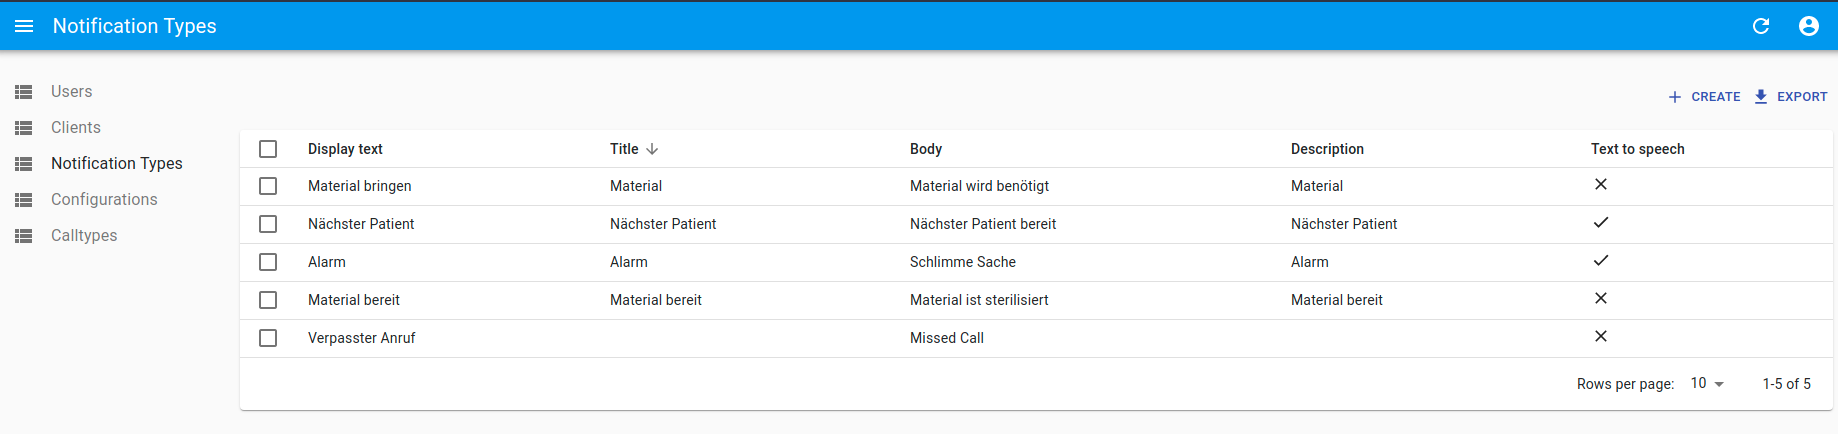
\includegraphics[width=\textwidth]{graphics/screenshots/admin_ui_notification_types}}
        \caption{Praxisruf Startseite}
    \end{minipage}
    \label{fig:AdminUI-Introduction}
\end{figure}

Die Grundlage für das entwickelte Praxisrufsystem wurde im Rahmen der Projektarbeit ''IP5 Cloudbasiertes Praxisrufsystem'' erarbeitet.
Im Rahmen des Vorgängerprojektes wurde bereits ein Praxisrufsystem mit eingeschränktem Funktionsunmfang entwickelt.
Die in diesem Projekt entwickelte Lösung ist eine Erweiterung des bestehenden Systems.
Das zuvor umgesetzte System unterstützt das Versenden und Empfangen von Benachrichtigungen.
Sprachsynthese für Benachrichtigungen und Sprachverbindungen für eine Gegensprechanlage konnten im Rahmen des Vorgängerprojektes nicht umgesetzt werden.
Die zentrale Aufgabenstellung für dieses Projekt war es, das System zu erweitern so, dass Benachrichtigungen vorgelesen und Sprachverbindungen aufgebaut werden können.
Die Bedienung des Praxisrufsystems soll weiterhin über eine mobile Applikation möglich sein.
Dazu soll eine neue, native iOS Applikation entwickelt werden.
Diese ersetzt die bestehende App und muss alle bestehenden Funktionen unterstützten.
Sie muss zudem Sprachverbindungen zu anderen Teilnehmern aufbauen und den Inhalt von Benachrichtigungen vorlesen können.

Wie in der Aufgabenstellung beschrieben, hat eine Marktanalyse im Vorfeld dieses Projektes gezeigt, dass bestehende kommerzielle Praxisrufsysteme veraltete Technologien einsetzten.
Diese Systeme sind aufwändig zu installieren und skalieren schlecht.
Sie können weiter nicht einfach in ein TCP/IP-Netzwerk eingebunden und über externe APIs angesteuert werden.\cite{aufgabenstellung}
Das im Rahmen des Vorgängerprojektes umgesetzte System löst diese Probleme bereits teilweise.
Mit dem Cloudservice bietet das System einen zentralen Dienst, welcher über eine Http Schnittstelle ansprechbar ist.
Diese ermöglicht die Verwaltung der Systemkonfiguration und stellt Benachrichtigung anhand der Konfiguration an relevante Empfänger zu.
Dadurch ist es einfacher möglich, das System in Netzwerke einzubinden, zu skalieren und neue Endgeräte anzubinden.
Das Vorgängersystem unterstützt aber noch nicht alle Funktionen, die ein Praxisrufsystem bieten muss.
Die meisten kommerziell erhältlichen Lösungen können als Gegensprechanlage verwendet werden\cite{aufgabenstellung}.
Ein vollständiges Praxisrufsystem muss deshalb unbedingt als Gegensprechanlage verwendet werden können.
Mit der Integration von Sprachsynthese für Benachrichtigungen kann sich das System weiter von bestehenden Lösungen absetzten.
Ein weiterer Schwachpunkt des Vorgängerprojektes ist die mobile Applikation.
Diese wurde mit einer geteilten Codebasis für iOS und Android entwickelt.
Im Fazit des Vorgängerprojekts wurde festgehalten, dass diese Applikation idealerweise neu als native Applikation entwickelt werden sollte.
Dadurch könne effizienter Betrieb, Wartung sowie Hardware- und Betriebssystemkomaptibilität langfristig gewährleistet werden.\cite{ip5}

Das umgesetzte System besteht aus drei Applikationen.
Der zentrale Cloudservice dient zur Verwaltung der Konfiguration und dem Vermitteln von Nachrichten zwischen Endgeräten.
Das Admin UI bietet eine Weboberfläche mit der die Konfiguration des Cloudservice verwaltet werden kann.
Mit dem Mobile Client bietet das System eine iOS App über welche Sprachverbindungen aufgebaut und Benachrichtigungen versendet werden können.
Für das Versenden von Benachrichtigungen, sendet ein Mobile Client eine HTTP Anfrage an den Cloudservice.
Der Cloudservice findet in der Konfiguration alle relevanten empfänger und leitet die Benachrichtigung an diese weiter.
Für die Zustellung von aus dem Cloudservice an Mobile Clients wird Firebase Cloud Messaging verwendet.

Für die Synthese von Sprachdaten wurde eine Anbindung an AWS Polly im Cloudservice implementiert.
Der Cloudservice bietet neue eine Http Schnittstelle, über welche Clients Sprachdaten für Benachrichtigungen beziehen können.
Durch diese Lösung müssen die Endgeräte die Anbindung an den Sprachsyntheseprovider nicht selbst implementierten.
Dies bietet den Vorteil das der Provider leicht ausgewechselt werden kann und dass die Anbindung von zukünftige Platformen übernommen werden kann.

\begin{figure}[h]
    \centering
    \begin{minipage}[b]{0.75\textwidth}
        \fbox{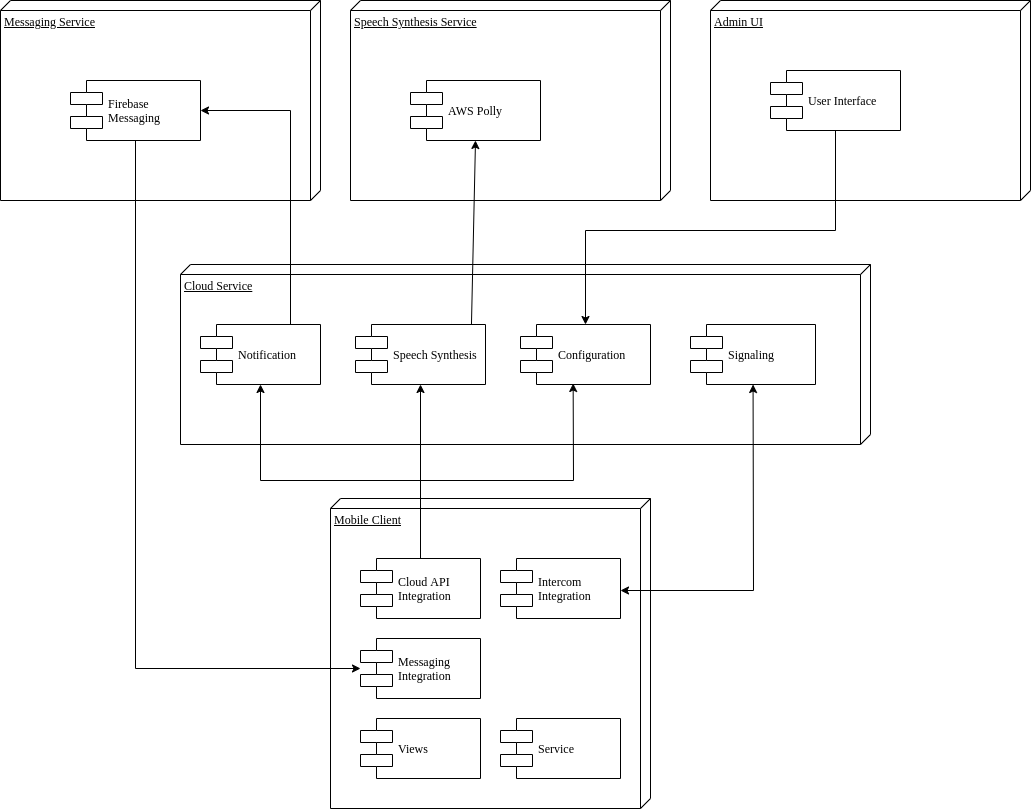
\includegraphics[width=\textwidth]{graphics/diagramms/Component_System_V02}}
        \caption{Systemarchitektur Praxisruf}
    \end{minipage}
\end{figure}

Sprachverbindungen zwischen Mobile Clients werden als Peer To Peer Verbindungen aufgebaut.
Diese Verbindungen wurden mit der Technologie WebRTC umgesetzt.
WebRTC steht für Web Real-Time Communication.
Dabei handelt es sich um ein Open Source Projekt, welches Echtzeitkommunikation für mobile Applikationen und Browser Applikationen ermöglicht.
Damit Peer To Peer Verbindungen zwischen Mobile Clients aufgebaut werden können, müssen diese Meldungen austauschen können.
Um dies zu ermöglichen, wurde der Cloudservice um ein Modul ''Signaling'' erweitert.
Dieses Modul bietet eine Websocketschnittstelle, über welche die nötigen Signalmeldungen ausgetauscht werden können.
Jeder Mobile Client der für Sprachverbindungen verfügbar ist, baut bei der Anmeldung eine Websocketverbindung zum Signaling Modul auf.
Über diese Verbindung sendet und empfängt er alle Signalmeldungen, die für den Verbindungsaufbau notwendig sind.

Im folgenden Bericht werden die erarbeiteten Konzepte und Resultate vorgestellt.
Zunächst werden Vorgehensweise, Projektplan und die Organisation des Projekts vorgestellt.
Anschliessend werden die Anforderungen, welche zu Beginn des Projekts definiert wurden, beschrieben.
Es folgt eine Technologie Evaluation für Sprachsynthese und Gegensprechanlage.
Dabei werden mögliche Optionen beschrieben und anschliessend eine begründete Entscheidung beschrieben.
Das darauffolgende Kapitel beschreibt das detaillierte technische Konzept für Funktionsweise und Architektur des Systems.
Es wird beschrieben, wie die Funktionen Gegensprechanlage und Sprachsynthese umgesetzt wurden.
Dabei wird insbesondere darauf eingegangen, wie die bestehende und neue Funktionen im neuen nativen Mobile Client integriert werden.
Weiter werden die notwendigen Abläufe, Kommunikationskanäle und Datenmodelle beschrieben.
Nach dem Konzept werden die Resultate zusammengefasst und die umgesetzten Ansichten des nativen iOS App abgebildet.
Am Ende der Arbeit stehen ein Fazit und Schlusswort mit Empfehlungen für das weitere Vorgehen.

\clearpage
